%!TEX program = xelatex

\documentclass[color=green,mathpazo,titlestyle=hang]{elegantbook}

\author{周涛}
\email{zhoutaoccu@163.com}
\zhtitle{叶不曾落\LaTeX{} }
\zhend{心的历险}
\entitle{Elegant\LaTeX{} Book}
\enend{Template}
\version{0.00}
\myquote{Victory won\rq t come to us unless we go to it.}
\logo{logo.pdf}
\cover{cover.pdf}

%green color
   \definecolor{main1}{RGB}{0,120,2}
   \definecolor{seco1}{RGB}{230,90,7}
   \definecolor{thid1}{RGB}{0,160,152}
%cyan color
   \definecolor{main2}{RGB}{0,175,152}
   \definecolor{seco2}{RGB}{239,126,30}
   \definecolor{thid2}{RGB}{120,8,13}
%blue color
   \definecolor{main3}{RGB}{20,50,104}
   \definecolor{seco3}{RGB}{180,50,131}
   \definecolor{thid3}{RGB}{7,127,128}

\usepackage{makecell}
\usepackage{lipsum}
\usepackage{texnames}



\begin{document}
\maketitle
\tableofcontents
\mainmatter
\chapter{文艺你说的}

只有当自己想去做一件事的时候才能把事情做好!拙笔虽拙,唯真得心。

\section{驻守,守望}
纪念那个球场,那个下午

熟悉的看台,开阔的视野,自从大一的拥簇和打闹

到现在暮然回首,自己近段的苍白

让我彳亍地毫无道理

没有预兆,瞬间两年过往~\\

我轻轻地走过,跑过,慢游过

旁边有人,没人

想象着自己要在跑道上追逐梦想,朝花夕拾

牵手走过段段

梦回大地希望满怀~\\
 
只是岁月太过匆匆,没有力气去掌控

指隙淌过,无声无息

论世事蹉跎,谈音乐电影,人生爱情

虽埋藏着不愿解开的伤

我积极,不怠慢~\\
 
靠不住的是别人的肩膀,寻得到的只能是被靠的来往

情感积累作响,也没法静下好好商量

人这个复杂的动物,没法用逻辑去猜想~\\
 
我独立于世,拾起还有的梦想

不苟言笑,对自己的心说一遍,我是BZTS

还记得那个学不成名誓不还的声音吗~\\
 
成名,淡泊明志,先行志,后得名

没想过什么时候能实现,只求自己回顾的时候能说声我真拼过

我对于别人没有丝毫优势

但我知道我缺什么

而且我能有目标去达成弥补的效果~\\
 
以前我会挖掘信息,成为引领信息的弄潮人

在别人面前我是智多星

那些炫耀的基础是我曾为此拼过,我想要别人对我不一般,我就要变得不一般

为此,我曾努力过,并为此感到满足~\\
 
如今我依旧在某些方面还能说话,但是面前已经狭隘到被人无视,被人嘲笑

思考是一个聪明人最爱做的事,而反省是最被受用的方法

做一个自信心爆棚的人,才会有更多的人知道我,我也就能真正的做好一个强我,而非那个被人忽视,视而不见的我~\\

少年强则国强,我强,才能扛起未来不可预知的世事无常~\\

--2015-05-04

{\color{thid}忍不住插个图!}

\begin{figure}[!hbtp]
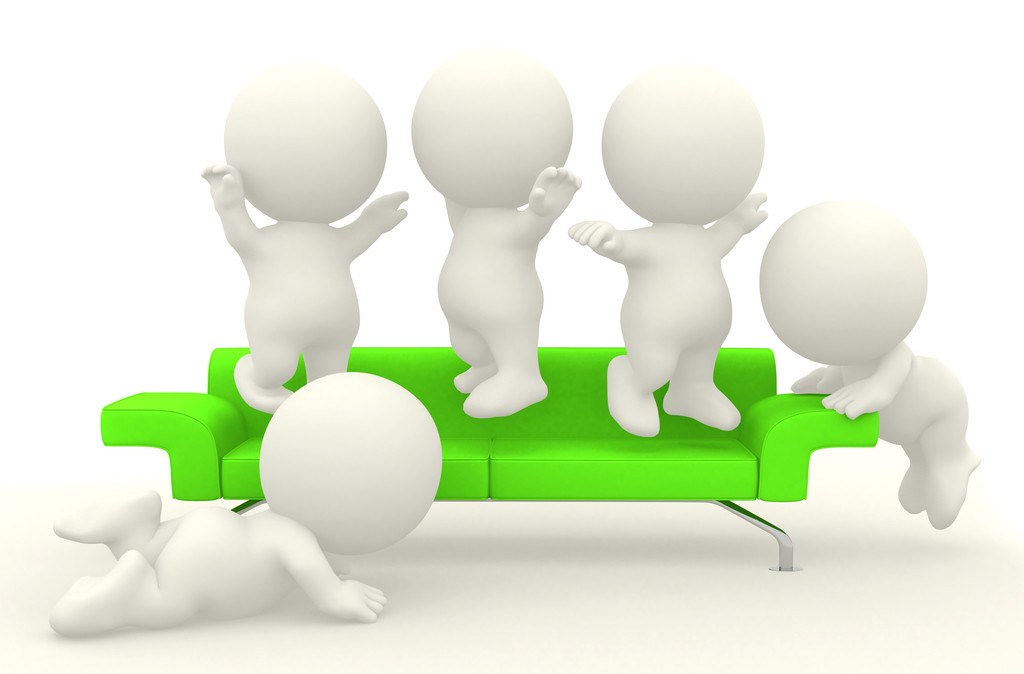
\includegraphics[width=0.8\textwidth]{happy.jpg}
\caption{Happiness,We have it!\label{figur:happy}}
\end{figure}

\section{时间可以疗伤}
时间可以疗伤,时间让人遗忘。时间可以掺淡,时间让人圆满。闻剑有感

时光确实一去不复返,但是它既然划过就有了它的光彩,生命的一次性也验证了它的唯一和特殊性。

有些情,随缘而来,随缘渐长,随缘而分,看似正常,实则微妙。世上没有永恒的朋友,只有永恒的利益。而即使利益冲突不再,情也一次消逝。所以所有友情爱情亲情也是一次性的,没有重来的笑话,那只是电视剧里的情节。所以我很重情,只要我们不相恨,那便见过聊过度过即有情,相识便是一次独有的经历。我也相信每个人都是有情有肉的人。故而备受内心的注重,因为有些经历会让你明白有些吹弹可破的变质的情那么容易发生在自己身上,为什么不去关注自己身边实诚的情,而要去发展所谓轰烈无比的花样情愫,遇见就是美好,人生最要好的朋友只能那么几个,多了不叫知己,叫花心。所以情浅请珍贵,情深请信赖,情当断则断。

时间可以清空记忆,重置情感是大家对时间最多的赞扬,因为一切都将过去。时间也是一种经历,满足你对世界的认识,对未来的构想,你的观念会变,你更完善,你更明白自己想要怎样的人生,你的圆满人生也就是你的利益宏图。所以有人更想要美好人生,故而忘记什么叫一种情义永流传,好吧,谈谈在利益下的情到底还有没有立足之地。

每个人追求人生圆满有错吗,每个人拓宽自己人脉有错吗,每个人提升认知变换人际圈忘了以前的浅情有错吗,每个人在为了自己的发展,利益,损害了情义又有什么大不了的?这些都没错,错就是错在你们并不是知己,还有对知己的要求。这是出问题,没得到解决,最终崩盘的原因。

既然时间让你阅历丰富,时间让你淡忘一些记忆,一些关于情义的记忆。不是知己,你怎么可能记人家一辈子。

既然你选择利益损害情义,又不会事先告诉别人你自己心里的想法,不想别人来帮忙解决。不是知己,你怎么保证每个人都在利益面前对你坦诚相待,跟你掏心掏肺。

所以知己的好处千万种,有了几个知己就好好保持沟通。情浅的情义在身边也就好好珍重,不要要求太高。如果本来就清浅的关系,又有知己的要求,那就作个陌生人吧,毕竟有容乃大,总有人给你想要感觉,不在现在,也许就在不久的将来。

(此文献给为情纠葛的人)

文:波涛鱼儿


\chapter{杂想片段}

\section{小感想}
\begin{enumerate}
	\item {\color{main}你可以不强,但是你认识的人一定要强。}古人说,人以类聚,物以群分。中国是个靠关系的社会, 中国关系网的重要性不言而喻,相对而言,欧美的关系文化比较淡,不会跟你说话的时候,谈到你的七大姑八大姨,你舅舅的大表哥的弟媳妇。中国的关系文化可以为你省下不少烦心事,甚至一步登天,当然,为了维持这个关系你得倾尽所有,你的不痛不痒,不闻不问,导致最后只有崩盘。这些关系让我又想起来了现在的朋友圈,不是我的思想呆板,固执,眼里只有黑暗,但确实这个社会从不心疼没有价值的东西。人与人之间最好的联系桥梁就是利益。没有永远的朋友,只有永远的利益。这是你经历了青葱岁月之后必须面对的事实。你可以在你同学成群,从小玩伴的QQ空间里,随手上传一张自拍,但你现在肯定不敢不加挑选,不加琢磨,不加修饰的在朋友圈里随便po一张你的普通生活照,甚至稍微low一点的景色图,都会让你觉得与当今整个朋友圈的氛围不搭。如今,成人的世界里需要树立形象,需要高端大气上档次,需要international,不入流的街边小巷,不入眼的黑脏胖矮,不着边际的爱好习惯,统统都被社会主流眼光扼杀在社交圈里。朋友圈里不再是为了分享生活体验,传播心得经验,而是流于炫耀,流于形式,可能自己满足感很高就够了,我的朋友圈我做主。对,你高兴就好!但是这就是我们想要的朋友圈吗,你的1000位好友,现在有10个一周内经常跟你说过几句心里话吗,有几个跟你不是套路而是踏实的交谈问候。没有!如今现实都太残酷了,每个人的生活都很艰难,都没有过多的精力,投入到那么伟岸的人际建设当中去。{\color{main}所以,请对你所交流的对象重视且珍惜,对那些虚无缥缈的关系忽略不计,人不要那么累,你的每笔人际交流都是投资,慎重且花心思。}
	\item  {\color{main}苦难是个好东西,从头到尾都是。}说起苦难,可以写很多篇议论文,但是现在大家可能都知道写,但都不想动手写,觉得,恩,你说的苦难理论都是对的,我无条件支持,我也懂得这个道理。好,我就来说说。首先要讲一个极端,一个顺风顺水的成功人士,没有经历过风浪,不懂得什么叫同舟同济,相濡以沫,遇到些许的挫折便会觉得全世界都在针对他,老天不公之类。而如果你经历过一些苦难,再遇到麻烦的时候就会坦然一些。这是从心理学角度来说明苦难其实可以说是一种抗压的经历,有了他心理承受能力大一些,当然,苦难的大小程度也对应你的心理素质强弱。其实越有资历的人,见识越多,按照成功失败比也可以推出其经历的苦难也是很多的。他们面对事物的发生,转折,跌宕起伏,哑然结束,全都经历过,所以他们对待人,事物都有种淡定从容的自信,这些能发生的结果我都预料过了。这是从人生经历上来看苦难其实就是一种阅历。见多识广的意思。苦难还有一种作用就是它确实能够让人意识到自己。伤口撒盐往往更刻骨铭心,苦难容易让人思考,让人沉淀,能够看清自己的薄弱之处,从而更加知道怎么去完善自我。苦难心酸的历程只有自己知道,自己体会,人们都善于表现自己光鲜有作为的一面,而苦难与心酸都藏在心底,等待有个懂你的人细细领会。苦难永跟随,到了该到的地方,自然你就看不到他了,只会留在你的回忆里。
	\item 
	{\color{main}高中确实是语文素养的巅峰,我从未质疑过。}高中语文老师每每苦口婆心地布置作业和作文的时候,都会说好好珍惜现在脑子里的古诗词,正反例,以后写文章可就没那么提笔就来了。确实,作文一直是我们最想鄙视的东西,考场作文,更是如八股文一般,残害广大青少年的心灵,高考竟然还不让写诗词作文,真是我大中华的悲哀,后世的悲哀。我们那时候崇尚自由,想要那种文笔自来,提笔生花的随意,想要思如泉涌,无拘无束的自由。那也许就是青春该有的样子。但是现在提笔忘字,捉襟见肘,也是笑煞旁人。每每写一个诸如入党申请书,年终大总结,就靠着百度上的随意搭配,自己的那些经历好像也有,但是记得不清楚,记得清楚有描述不清,描述清楚又用词不当,能想出几个词,又没有时间。我现在觉得,中华文字一个锻炼记忆力,另外锻炼逻辑能力。我们懒于文字的描述,其实就已经养成了思维的懒惰,我们倾向于复制粘贴,而不再习惯一纸空白的思绪挥洒。当然这确实是网络社会带来的负面影响,因为,大家都最求短小精悍,简单简约,速效速度,酣畅淋漓。大段文字看不下去,长篇大作没心情写,慢慢地自己的真实表达掩于心底,口头书面却总戛然而止。所以说高中语文的训练了大家的用词造句能力,而大学工作,则教会大家怎么把这种最基本的能力退化。说来可笑,但这个趋势势不可挡,真的现在能长篇大论800字,并且头头是到,让人心服口服,原意去写的少,能写出来的更少。所以说,语文这东西不是那么强硬的指标,但是真的能体现一个人的素养,反映一个人思考人生的态度,表达自我的真实与自然。
	\item {\color{main}仪式感成为未来人群最为注重的生活要素。}仪式感是什么?大家会想到婚礼,喜宴,朝拜,信仰,使命。这些仪式感强烈的东西给人一种震撼,高大上的感觉,其中不乏认真筹备,实施,落下帷幕。仪式都有它的一套流程,它的故有历史感,认同感,渗入骨髓血液,让人无法拒绝。这些都是传统的仪式感,再举几个粟子。看电影。以前看盗版光碟,盗版资源是一个时代的印记,弄个DVD,买张几块钱的电影光碟,虽然画面模模糊糊,声音嘈嘈杂杂,但总是乐在其中,不免觉得自己像人生赢家一样,比影院中的电影真是好上100倍。但是随着人们生活水平的提高,我们越来越注重生活品质,电影院看电影成为一种生活方式。为什么呢?不仅因为视觉效果,声音质量好,同时因为在电影院看电影有一种仪式感在里面,成为情侣,家庭的消费习惯。仪式感的代入赋予了电影院一个系统,有流程,有环境搭建,有组织纪律 的一个固定仪式,而不是随随便便,网上download一下,就可以想在哪看就在哪看,想和谁看就和谁看。它是一套规范的流程,需要预定时间,地点,场次,还要在看电影的时候不能打扰别人,也不能在看电影的时候吃火锅,麻辣烫,或者上厕所。因为固定套路,这个仪式感不知不觉地提升了整个看电影的逼格,你也会打心底地重视这场电影,毕竟这是花钱占座才得到的,得认真看呀。仪式感就这样深深地吸引了你,所以你开始收藏唱片CD,你开始听那种复古的留声机,你开始做一些复杂但不乏味,简单但又费心的具有仪式感的事情,觉得这样才是有品质的生活。这是为什么呢?其实没有对比就没有伤害,现在网络的发达使得以往一些觉得世俗别扭不方便的东西变得极具仪式感。现如今,网上电影一大堆,你想看吗?额,看时间,兴许脑门一热,可能会过去看一看。数量多意味着不重视,没吸引力。现在外出旅游,看到有排长龙的小吃摊,果断要去排一排,排队也是一种风景嘛。排队说明这好吃啊。虽然人多,但这仪式感足啊。以后想排队还没有机会了呢。确实,生活过程中需要适当增加仪式感比较强的内容,生活也才更有情调,不然全都高效率了,人活着干吗啊。没事去自己做一顿饭,学做个面包,学做碗面条,多有仪式感,这种掺杂了仪式感的慢生活也许就是我们苦心追求的吧。
	\item 
	{\color{main}你可以有很少,但是你不能没有。}小时候考试前,老师都会千叮嘱万嘱咐,考试的时候一定要带笔,橡皮,尺子,结果你带了两三支铅笔,圆珠笔,修正笔,害怕不够墨。大学期间,你抱怨,怎么要考这么多证啊,到底有什么用,有证就能找到好工作吗?其实其中的道理是一样的,有总比无要好。不是拥有很多就很好,而是说你没有肯定差。其实这个我联想到的就是世界观,见世面。小的时候看了关于地球在宇宙中地位的科普漫画,觉得世界真小,我想出去看看。长大了,发现世界还是挺大的,看一辈子可能都看不完。人的眼光是会变的,随着认识面的拓展和深度的加深,我们总是以一个过来人的姿态去回顾,但是总是忘了,有人也在回顾我们。活到老,学到老,成为了大家学习的座右铭。世界上发生的事情太多,虽然你能感受,你却无法把他们一一记下,其实你感受到了就够了。其实如今的信息社会爆炸,随随便便给你一个堆信息,你可以选择不管不问,也可以选择加以思索的取用。知识从来不嫌多,知乎上常常有一些问题是问,什么时候让你感觉高数特别有用?这些问题就应证了,知识面越宽,你看到的世界可能就不一样了。现在人们阅读习惯丧失,同时好奇心也没了主人,都不愿意成为第一个吃螃蟹的人,不愿意去尝试一些新事物,给自己的生活增加一些新能量。真的尝试新的东西,并不需要你精通,可能你只需知道他在那就行了。一位女子抱怨自己高考物理都没及格,根本无法理解什么罗七八糟的量子学,我看它有什么用?物理学家回答她说,你不需要弄清楚它的原理,但你要知道它的存在,并在心中,心生敬畏即可。所以,人生漫漫,不论烟花易冷还是残风弄影,兴趣使然,就赶紧去看看,也许那块未开垦的田地,就有你一席之地。
	\item 
	{\color{main}写作的技能永远不会过时。}小时候的日记,周记,作文,都是自我总结自我表达的一种方式,现在的人都觉得写这些东西有什么用,还不如去敲点代码,写点论文,写的又不能发表,又不能发小说成四大才子,稿费没稿费,还TM要一个个敲,对,写了我也不会再拿出来看,算了,还是回去洗洗看看剧吧。我记得之前看过一篇文章,说美国的小孩需要写很长的论文,可能布置一个主题,各自发挥,然后组织资料,以及自己的想法,最终得出一个论文。上交的论文任何地方引用的地方都要标记,表示对原作的尊重,然后其余要保证是自己的想法。以前看到这里我可能会认为,美国教育就是重视创新啊,找资料得多费时间,还要弄点名堂出来,写点自己的理解,这样就是自己的独创的啊,而且知道哪些是别人的,哪些是自己的,小孩也牛逼啊,能憋出出这么多字,也是大白话全拿出来用啊。现在看来,人家鼓励的不是你你能出多少成果,多少创新独到的想法,而是鼓励你去自己思考,自己表达,从不断的模仿别人,提高自己的表达,清楚自己要表达什么,可能老师根本就不会在意你再这个主题提出多牛逼的创新,而是在乎你现在的写作水平,你的内心想法到底是什么思想状况,是幼稚还是稍微地成熟。宁外写作的过程其实是一个不断反省自己的过程,不断思考自己的过程。你会发现让你说一句话可以不加思索,但是让你写篇文章,你会字斟句酌,想想这个是不是对了河里了,是不是符合实际情况,是不是语法对了,写出来是不是多余了?会有一个不断修正的作用。
	\item 
	{\color{main}每件成功或者美好的事都是有原因的。}侥幸这种东西存在,但是人生的考验太多,其实已经基本把侥幸的几率降得很低了,所有学会尊重每个有所成就的人,同时感谢别人为你所做的。天上掉馅饼只存在支付宝扫红包,不然可能会砸得头流血。人如果为你做了什么一个是因为它爱你,一个是因为它需要你反馈或者以后反馈给他。利益是人与人之间基本的条约,不要想着别人就是无赖,这么死皮懒脸对自己好,对自己关心,好需要反馈,否则就是感情的终结者。这就是老一辈之间人情的重视可见一斑,现在年轻人崇拜的那种自由,佛系,都是那种对于这种好坏无所谓的态度,我感觉还是躲不了的这个准则,只是时候未到。时间功夫唯快不破,人情还多为最。
\end{enumerate}


\chapter{读书笔记}

\section{傲慢与偏见}


\begin{conclusion}
看到一则小幽默,是这样说的:{\color{main} 别人都关心你飞的有多高,只有我关心你的翅膀好不好吃!}说多了都是泪啊!
\end{conclusion}

\end{document}
